%----------------------------------------------------------------------------------------
%	PACKAGES AND OTHER DOCUMENT CONFIGURATIONS
%----------------------------------------------------------------------------------------
\documentclass{beamer}

\usepackage[utf8]{inputenc} % to encode the document so that we can use more caracters (like Latin ones)

\usepackage[normalem]{ulem}
\usepackage{ragged2e}
\usepackage[absolute,overlay]{textpos}

\usepackage{mathtools}
\usepackage{amsmath}
\usepackage{bm}
\usepackage{stmaryrd}
\usepackage{cases}

\usepackage{graphicx}
\usepackage{float}
\usepackage{caption}
\usepackage{subcaption}

\usepackage{algorithm}
\usepackage{algorithmic}

\usepackage{amsthm}
\newtheorem{thm}{Theoreme}

\setbeamersize{text margin left=0.2cm}
\setbeamersize{text margin right=0.2cm}
%----------------------------------------------------------------------------------------
%DOCUMENT
%----------------------------------------------------------------------------------------

	
\setbeamertemplate{footline}[frame number]
	
\begin{document}
	
	%Title page
	\title {Récapitulatif Thèse, 18/02/13}
	\author {Mathilde Boissier}
	\frame{\titlepage}
	
	%Table of contents
	\begin{frame}
		\frametitle{Plan}
		\tableofcontents
	\end{frame}

%First section : Compute the shakedown limit
	\section{Projet 1 : pour chaque couche, chaque composante connexe est un cercle}
	
	
	\begin{frame}
		\frametitle{Objectif}
		
		\begin{columns}
			\begin{column}{0.45\textwidth}
				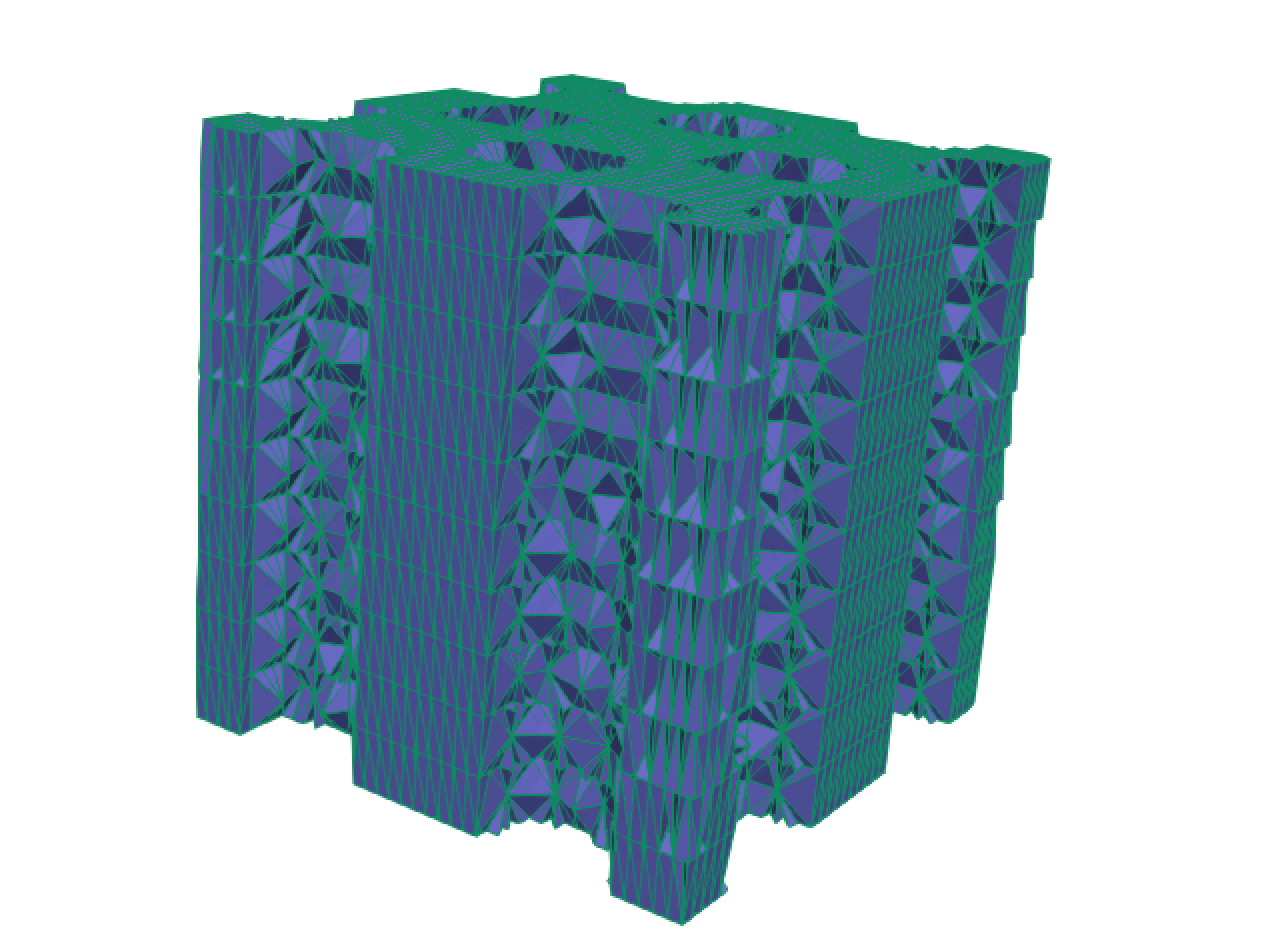
\includegraphics[width=0.8\textwidth]{Ini2}
			\end{column}
			\begin{column}{0.45\textwidth}
				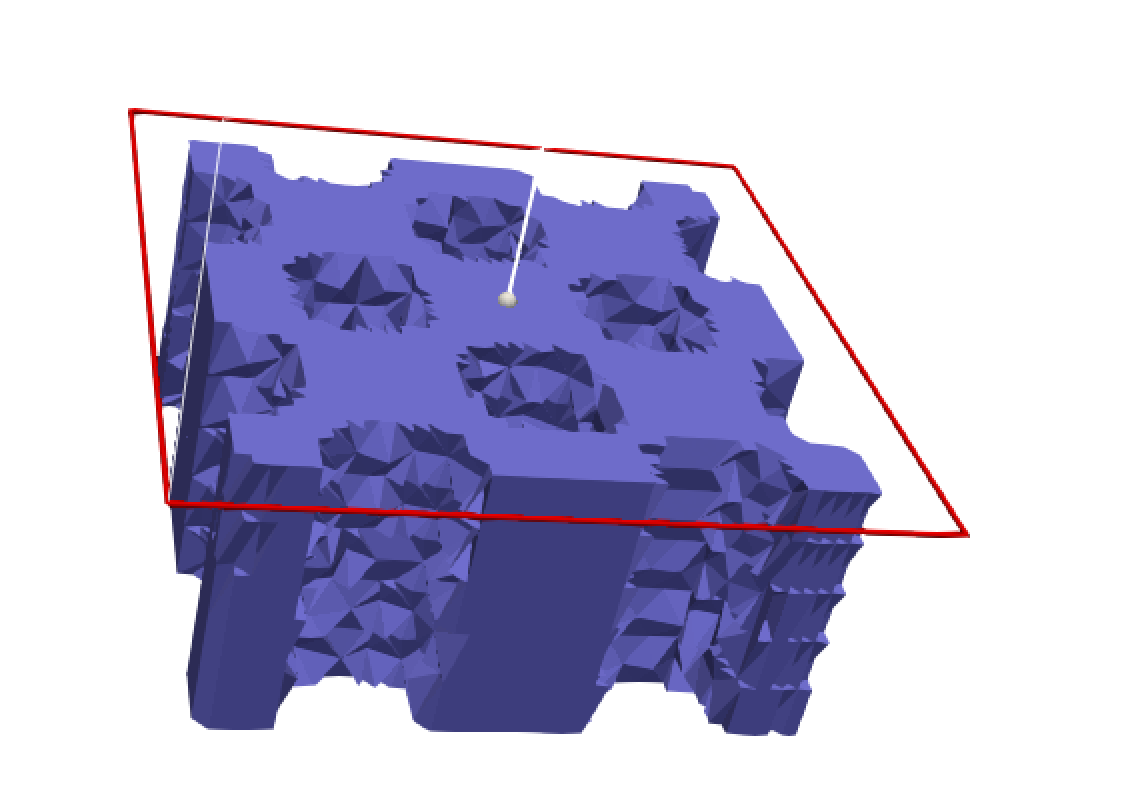
\includegraphics[width=0.8\textwidth]{coupeIni2}
			\end{column}
		\end{columns}
		
		\begin{columns}
			\begin{column}{0.45\textwidth}
				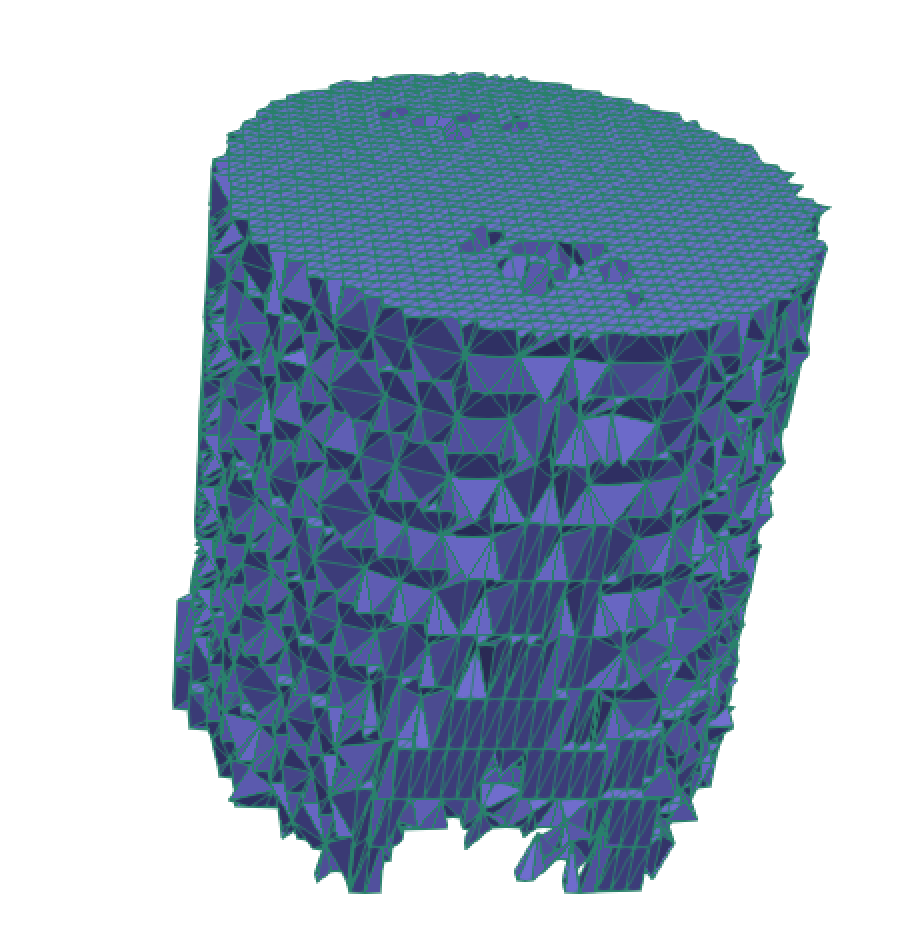
\includegraphics[width=0.8\textwidth]{Ini2Cercles}
			\end{column}
			\begin{column}{0.45\textwidth}
				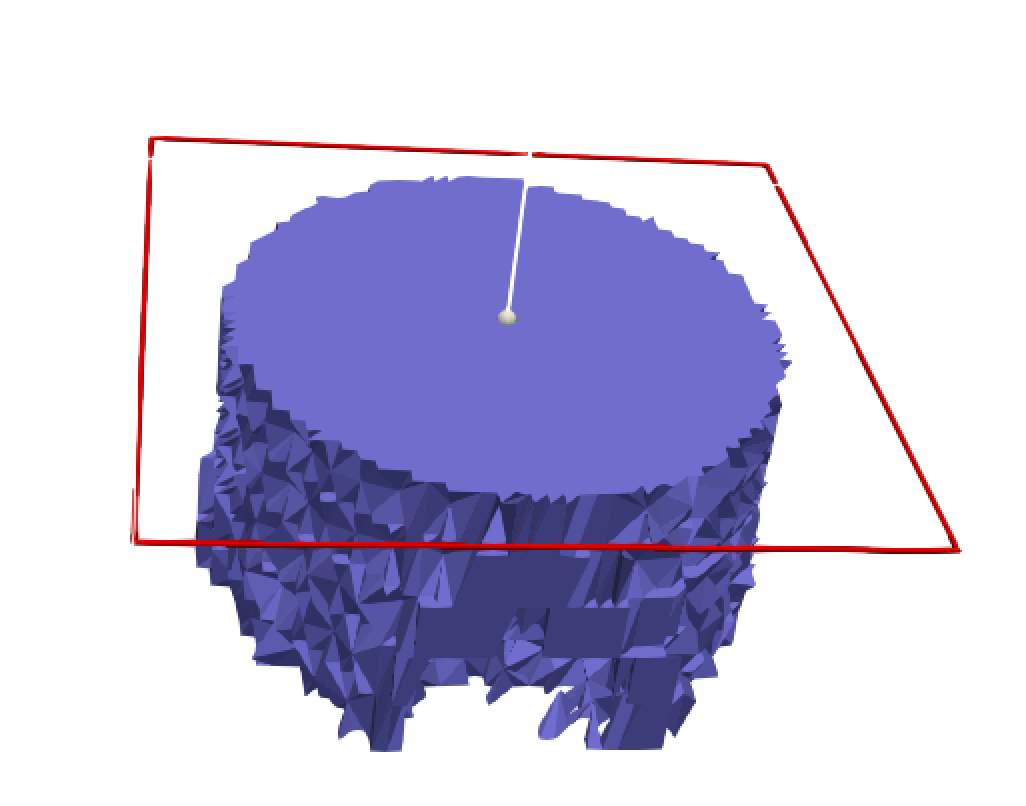
\includegraphics[width=0.8\textwidth]{coupeIni2Cercles}
			\end{column}
		\end{columns}
	\end{frame}
	
	
	\begin{frame}
		\frametitle{Maillage, levelset et elasticité}
		\begin{columns}
			\begin{column}{0.45\textwidth}
				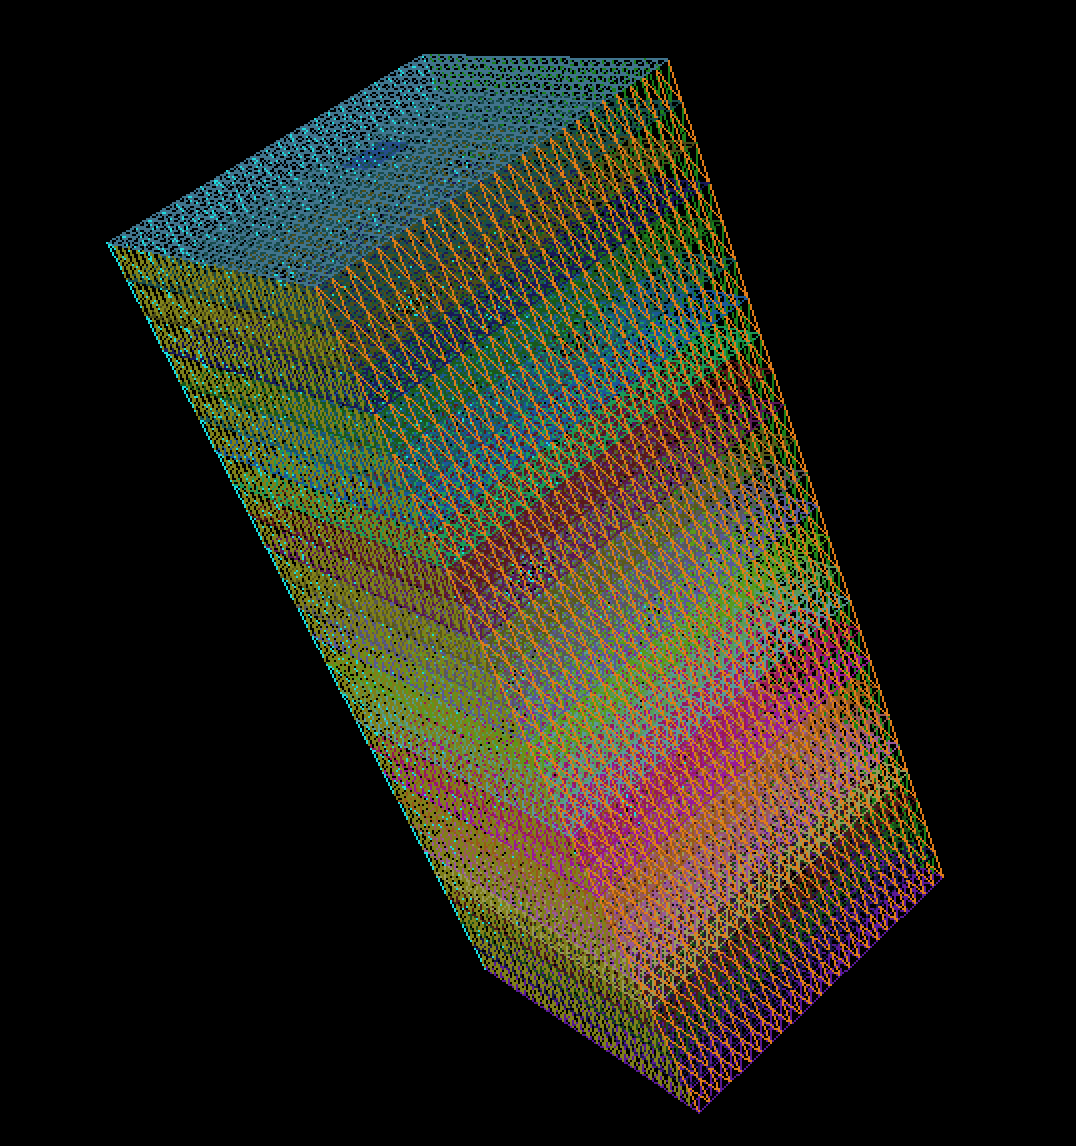
\includegraphics[width=0.8\textwidth]{mesh}
			\end{column}
			\begin{column}{0.45\textwidth}
				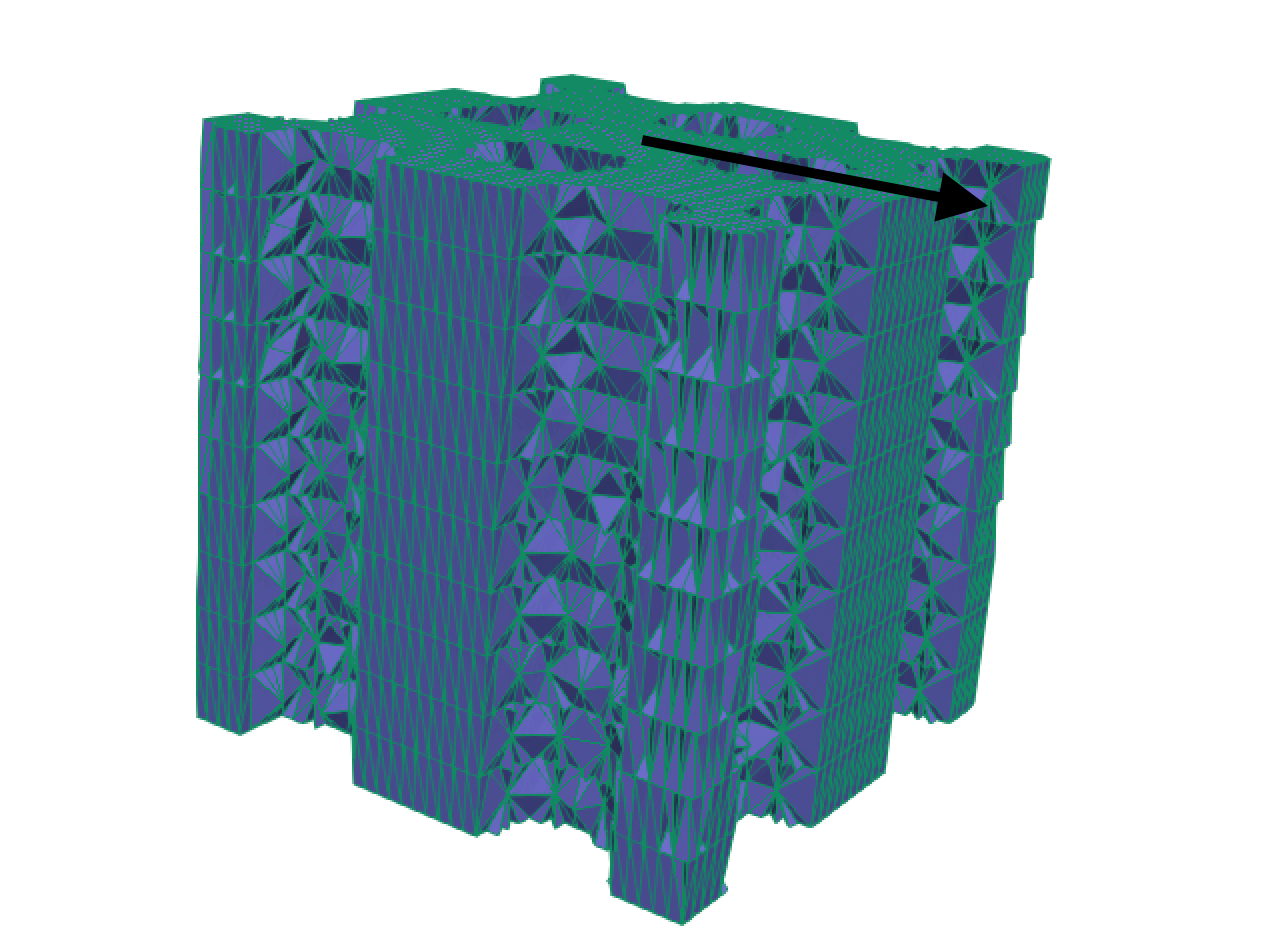
\includegraphics[width=0.8\textwidth]{Forces}
			\end{column}
		\end{columns}
	\end{frame}

	\begin{frame}
		\frametitle{Cercle Modèle}
		Pour chaque section, le "cercle objectif" est celui dont :
		
		\begin{itemize}
			\item L'aire correspond à l'aire de la section,
			\item Le centre correspond au barycentre de la section.
		\end{itemize}
		
		On cherche alors à minimiser 
		\begin{equation}
		\label{eq:defC1}
		\int_{\partial\Omega\cap (z=h)}d_{\mathcal{C}(\Omega\cap (z=h))}(s)^2ds
		\end{equation}
		avec 
		$
		\label{eq:explicitdist}
		d_{\mathcal{C}(\Omega\cap (z=h))}(x)=\sqrt{\Bigg(X(x)-\frac{\int_{\Omega\cap (z=h)}X(x)dx}{\int_{\Omega\cap (z=h)}dx}\Bigg)^2+\Bigg(Y(x)-\frac{\int_{\Omega\cap (z=h)}Y(x)dx}{\int_{\Omega\cap (z=h)}dx}\Bigg)^2}-\sqrt{\frac{\int_{\Omega\cap (z=h)}dx}{\pi}}
		$
		
		D'où la contrainte (transformée ensuite en somme sur chaque section -> voir maillage):
		\begin{equation}
		\label{eq:constraint2}
		P(\Omega)=\int_{0}^{H}\int_{\partial\Omega}\delta_h(x)dist(\Omega,h,x)^2dxdh
		\end{equation}
	\end{frame}
	
	
	\begin{frame}
		\frametitle{Optimisation}
		
		$\min_{\Omega} J(\Omega)=l_{cply}\textrm{Compliance}(\Omega)+l_{vol}\textrm{Vol}(\Omega)+l_{cercle}P(\Omega)$
		
		\vspace{2cm}
		
		Descente de gradient classique. Les coefficients sont fixés au départ et ne bougent pas.
		
	\end{frame}
	
	\begin{frame}
		\frametitle{Résultats}
		\begin{itemize}
			\item Force Centree, $l_{Cply}=1,\,l_{vol}=0,\,l_{cercle}=10$
			\item Force Centree, $l_{Cply}=1,\,l_{vol}=1,\,l_{cercle}=10$
			\item Force Non Centree, $l_{Cply}=1,\,l_{vol}=1,\,l_{cercle}=5$
			\item Force Non Centree, $l_{Cply}=1,\,l_{vol}=10,\,l_{cercle}=5$
		\end{itemize}
	\end{frame}
	
	\begin{frame}
		\frametitle{Pour la suite}
		
		\begin{itemize}
			\item D'abord élasticité seule pour avoir une structure avec des barres fines puis elasticite+cercles afin que les composantes connexes des sections de chaque barre soient circulaires.
			
%			\vspace{1cm}
			
			\begin{itemize}
				\item Lagrangien pour l'élasticité seule
			\end{itemize}
			
			\vspace{1cm}
			
			\begin{columns}
				\begin{column}{0.45\textwidth}
					pas de contrainte d'advection sur la frontière de Dirichlet :
					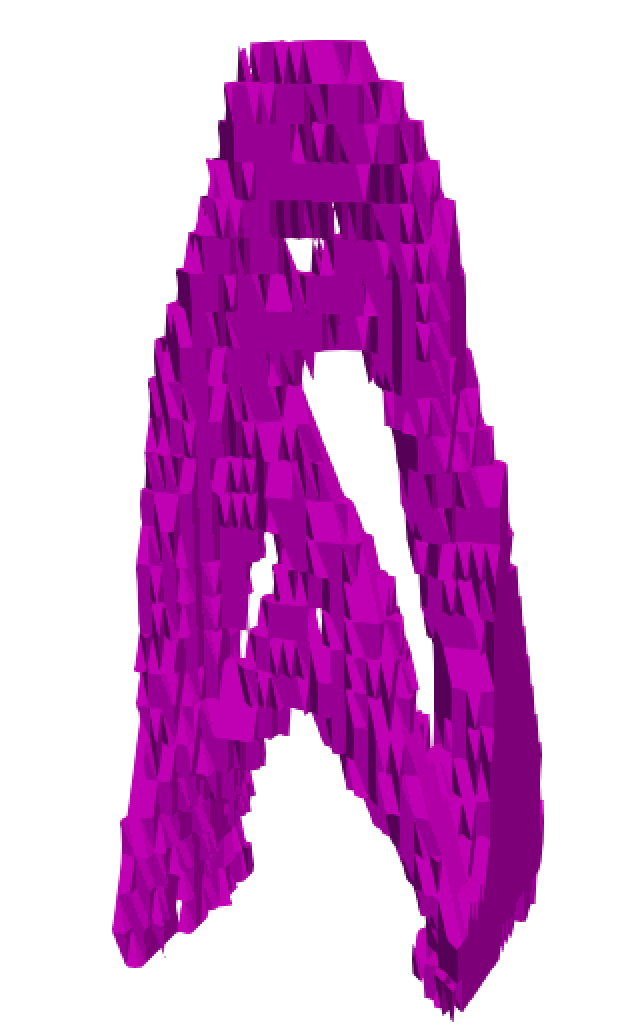
\includegraphics[width=0.6\textwidth]{elastSeule1}
				\end{column}
				\begin{column}{0.45\textwidth}
						Advection interdite aux coins de la frontière de Dirichlet
					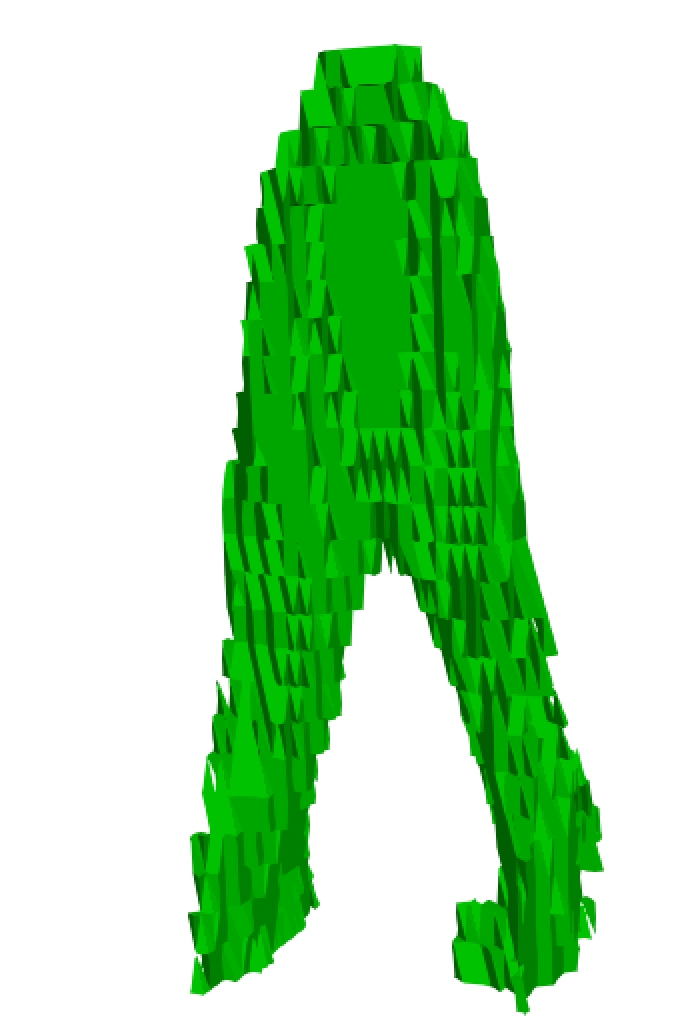
\includegraphics[width=0.6\textwidth]{elastSeule2}
				\end{column}
			\end{columns}
			
		\end{itemize}
		
	\end{frame}
	
	
	\section{Projet 2 : trajectoires de lasage}
	
	\begin{frame}
		\frametitle{Modèle Physique}
		
		\begin{equation}
		\label{eq:ChaleurNormale}
		\left\{
		\begin{array}{ll}
		\Big(\rho\partial_t T+\lambda T-div(\lambda\nabla T)\Big)=Q(\Delta L)& \textrm{in\,}(0,t_F(\Delta_L))\times D \\
		(\lambda\nabla T).n=-\beta(T-T_{ini}) & \textrm{in\,}(0,t_F(\Delta L))\times \Gamma_N \\
		T=T_{ini} & \textrm{in\,}(0,t_F(\Delta L))\times \Gamma_D \\
		T(0)=T_{ini} & \textrm{in} \Omega
		\end{array}
		\right.
		\end{equation}
		
	\end{frame}
	
	
	
	\begin{frame}
		\frametitle{Selon les lignes de niveau}
		
		\begin{itemize}
			\item Changement de phase quand 80\% de la puissance du laser est passée sur le point. Changement de phase instantané. Pas de frontière de Dirichlet.
			\item Paramètres :
			\begin{itemize}
				\item $\rho_{poudre}=450*4000;$, $\rho_{solide}=450*8000$
				\item $\lambda_{poudre}=0.25;$, $\lambda_{solide}=15.$
				\item $T_{ini}=0$
				\item $\beta=1000$
				\item $P_{laser}=768000*10^4$
			\end{itemize}
		\end{itemize}
		
		Résultats :
		\begin{itemize}
			\item Etoile : lignes de niveaux -0.05 et -0.4 
			\item Haricot : lignes de niveaux -0.05 et -0.4
			\item Haricot : ligne de niveau -0.3
		\end{itemize}
		
	\end{frame}

	\begin{frame}
		\frametitle{Simulation de trajectoires}
		
		\centering
		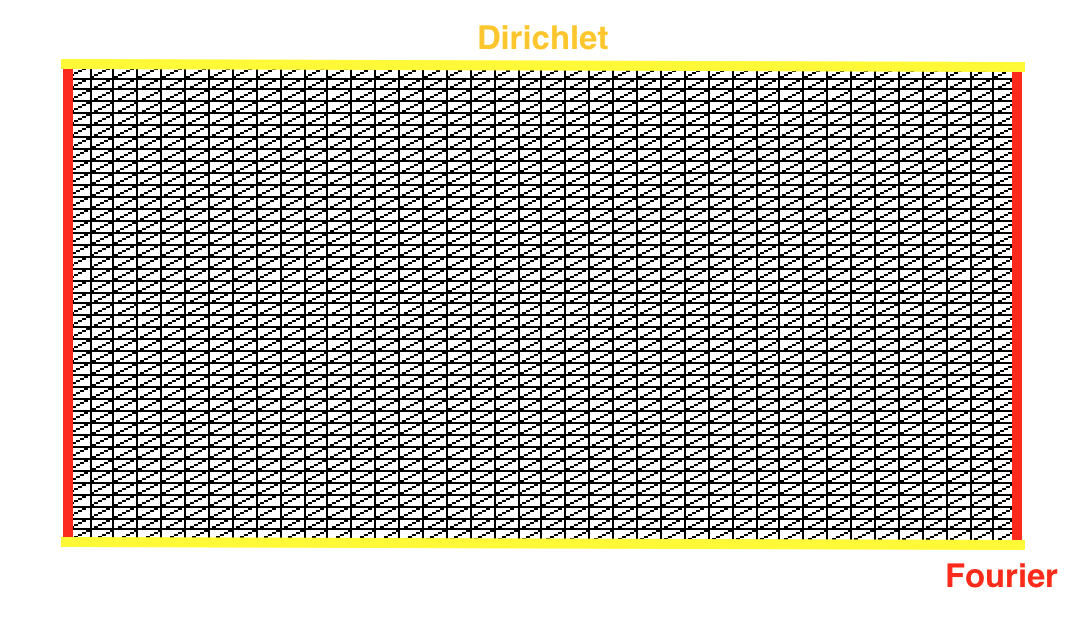
\includegraphics[width=0.5\textwidth]{rectangleTraj}
		
		\begin{itemize}
			\item Lignes droites
			\item Zig-zag
		\end{itemize}
		
	\end{frame}
	
	\begin{frame}
		\frametitle{Optimisation de la distance entre deux lignes, trajectoire en ligne droite selon (0x)}
		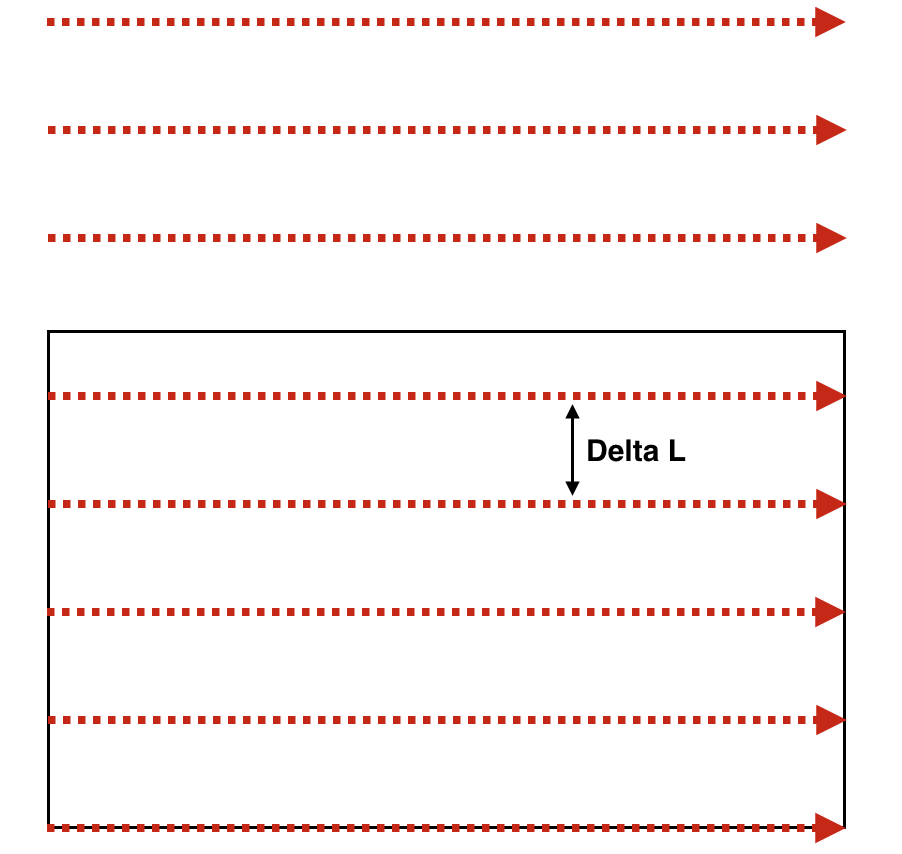
\includegraphics[width=0.7\textwidth]{lignesDroite}
	\end{frame}
	
	\begin{frame}
		\frametitle{Optimisation de la distance entre deux lignes, trajectoire en ligne droite selon (0x)}
		\begin{itemize}
			\item On souhaite que l'intégralité du rectangle soit solidifié. Fonction objectif :
			
			\begin{equation}
			J(\Delta L)=\int_{\Omega}\Bigg[\Bigg(\Big(\int_{0}^{t_F(\Delta L)}|T|^rdt\Big)^{\frac{1}{r}}-T_{fu}\Bigg)^-\Bigg]^2dx
			\end{equation}
			
			\item On ne veut jamais, en aucun point, dépasser une température sup. Contrainte :
			
			\begin{equation}
			\label{eq:contrainte}
			C(\Delta L)=\int_{0}^{t_F(\Delta L)}\int_{\Omega}[(T-T_{sup})^+]^2dxdt-\textrm{tol}_{sup}
			\end{equation} 
			
		\end{itemize}
	\end{frame}
	
	\begin{frame}
		\frametitle{Résultats}
		Valeurs utilisées :
		\begin{itemize}
			\item $\rho_{poudre}=450*4000;$, $\rho_{solide}=450*8000$
			\item $\lambda_{poudre}=0.25;$, $\lambda_{solide}=15.$
			\item $T_{ini}=30$
			\item $\beta=1000$
			\item $P_{laser}=768000*10^4$
			\item $T_{phase}=500$, $T_{sup}=850$
		\end{itemize}
		
		Changement de phase quand $T>T_{phase}$.
		
		\vspace{0cm}
		
		Ne fonctionne pas encore complètement. Il faut :
		
		\begin{itemize}
			\item Comprendre cette attitude bizarre de la vitesse quand on éteint la source.
			\item Fixer un temps maximal supérieur au temps nécessaire pour parcourir la trajectoire et éteindre la source quand elle sort du rectangle.
			\item Remplacer le pas fixe (pour l'instant fonctionObjectif=objectifPhase+coef*Contrainte, avec coef fixe). 
		\end{itemize}
		
	\end{frame}
	
	\begin{frame}
		\frametitle{Pistes pour la suite}
		\begin{itemize}
			\item Décomposer la trajectoire en segments de droite pour pouvoir faire la même chose qu'avant sur les isolignes.
			\item Optimiser la vitesse pour avoir la meilleure physique possible.
			\item Optimisation multiparamètres avec tout ce qui ne concerne pas directement la trajectoire de lasage : puissance du laser, vitesse, écartement entre les lignes... + quelles lignes en premier... Le tout à partir de biblio.
			\item intégrer d'autres trucs type wobbling...
		\end{itemize}
	\end{frame}
\end{document}

	